\chapter{\sf Results}\label{ch:results}

This chapter presents the results of our numerical investigation into nucleation in the PFC model. We first present results for model parameters that follow the recommended noise amplitude given by the authors of \cite{kocher16}, as mentioned in section \ref{sec:pfc_dynamics}. We analyze these results in the presumed late-time asymptotic limit for which we obtained the CNT-predicted behavior of the nucleation rate and incubation time. We then use the numerical methods developed in sections \ref{sec:num_wave} and \ref{sec:num_testnuc} to examine the early formation shape and behavior of solid grains. Finally, we present further results under relaxed model parameter choice, to showcase nucleation dependence on noise amplitude.


%%%%%%%%%%%%%%%%%%%%%%%%%%%%%%%%%%%%%%%%%%%%%%%%%%%%%%%%%%%%%%%%%%%%%%%%%%%%%%%%%%%%
\section{Nucleation rates and incubation times}\label{sec:res_longtime}

A total of six data sets where obtained. Each data set consists of the averaged results of 50 to 150 simulation runs. All data sets had fixed PFC model parameters $n_o=0.207$, $B^x=0.4$, and $N_a=0.04$. The effective PFC temperature $\Delta B$ increases between the data sets, chosen to be $\Delta B=0.16500 + 0.00025\epsilon$ for $\epsilon$ an integer from 0 to 5 corresponding to the six sets in order from first to last. The noise amplitude $N_a$ was chosen within the recommended range corresponding to the other parameters as given in \cite{kocher16}, bearing in mind that these authors' results show that the variation range of $\Delta B$ between the data sets is too small to warrant a change in $N_a$ between the sets.

The parameters chosen for these runs place the simulated systems below their solidus (at $\Delta B \approx 0.1685$ for the chosen $n_o$ and $B^x$) on their phase diagram, and above their instability curves (at $\Delta B \approx 0.1642$). The range of $\Delta B$ was chosen such as to allow appreciable amounts of nucleation to take place in a reasonable amount of computational time, while remaining above the instability curve. We note that this range is small relative to the range between the instability curve and the solidus, and that the range lies closer to the instability curve than the solidus, indicating that the systems are greatly undercooled below their freezing point for nucleation to occur at noticeable rates. While this might be a result of making the PFC model's equations dimensionless, there is some precedence in physical systems for such homogeneous nucleation behavior. For example, in the absence of heterogeneous nucleation, water is known to remain liquid at temperatures of $235K$ and below \cite{mason58,jeffery97}. See also \cite{hoyt_phasetransf}, where an estimate for the variation of $J_{ss}$ with temperature is obtained using realistic values for an alloy. This estimate predicts that the homogeneous nucleation rate is undetectable before a specific temperature more than $100K$ below the alloy's freezing point, yet the rate rapidly increases beyond that specific undercooling temperature, similar to the behavior our results will show. Such undercooling behavior in alloys has also been observed experimentally \cite{provatas_coms2}.

Figure \ref{fig:res_I_datasets} plots the post-critical nuclei densities $I^*(t)$, corresponding to equation \ref{eq:nuc_crit_numdens}, for the first 5 sets. The sixth set, with $\epsilon=5$, is not visible on that figure's scale. We observe that the early portion of these curves resembles the form predicted by CNT, such as in figure \ref{fig:nuc_rates_fixedinc_b}, except that it is unclear whether the linearly increasing parts of these curves reach the true asymptote before tapering off to a constant value at late times due to the system fully transitioning to solid.

\begin{figure}[!h]
	\centering
	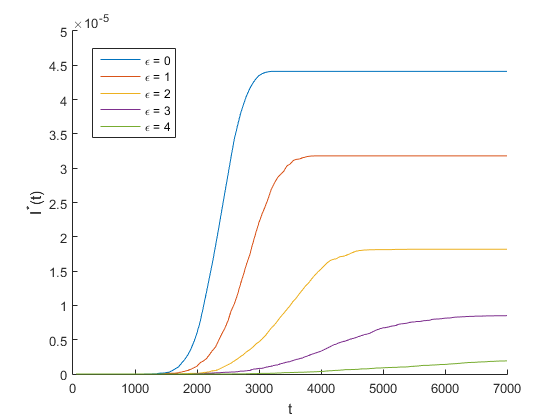
\includegraphics[width=0.7\textwidth]{fig_res/res_I_datasets}
	\caption{The post-critical nuclei densities for data sets $\epsilon=0$ to $\epsilon=4$.}\label{fig:res_I_datasets}
\end{figure}

\begin{figure}[!h]
	\centering
	\subfloat[]
	{
		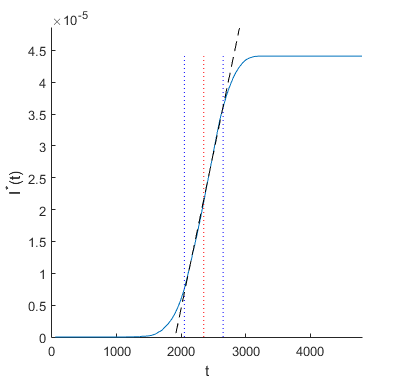
\includegraphics[width=0.5\textwidth]{fig_res/res_I0}
	}
	\subfloat[]
	{
		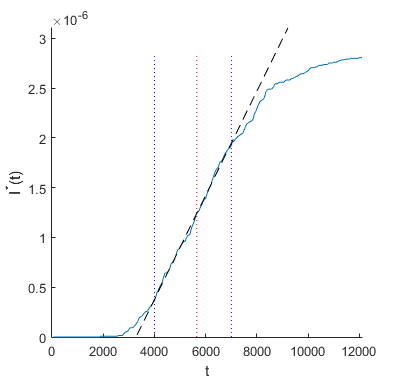
\includegraphics[width=0.5\textwidth]{fig_res/res_I4}
	}
	\caption{The geometric construction used to obtain $J_{ss}$ and $t^*$. The vertical blue dotted lines indicate the range of time taken to correspond to the asymptote. The dashed black line is the linear fit over that time range. Also shown as a vertical red dotted line is the time at which 10\% of the initial liquid volume has solidified. (a) Data set $\epsilon=0$, giving $J_{ss}=(4.9\pm 0.1)\times10^{-8}$ and $t^*=1910\pm 70$. (b) Data set $\epsilon=4$, giving $J_{ss}=(5.23\pm 0.08)\times10^{-10}$ and $t^*=3280\pm 90$. The errors on these values are from the uncertainty on the linear fit.}\label{fig:res_I_datasets_examples}
\end{figure}

We obtain the steady-state rate of nucleation $J_{ss}$ and the incubation time $t^*$ by the geometric construction described in section \ref{sec:nuc_fopl_sol}, taking as assumption that the linear part of each data set's $I^*(t)$ corresponds to the CNT-predicted asymptote. As a check for whether the assumption of asympoticity is sound, we also obtain for each data set the fraction of the initial liquid volume that has transitioned to solid as a function of time. We find that in all the data sets, only 10\% of the total liquid volume has solidified by the time approximately half of all nuclei have appeared. As the $I^*(t)$ curves have already entered the linear regime before that time, this suggests that the liquid has not yet been significantly depleted in the time range we assume to correspond to the asymptote. Figure \ref{fig:res_I_datasets_examples} demonstrates the geometric constructions for two of the data sets.%, as well as the time at which 10\% of the liquid volume has solidified.

\begin{figure}[!h]
	\centering
	\subfloat[]
	{
		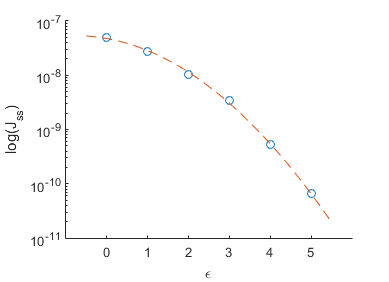
\includegraphics[width=0.5\textwidth]{fig_res/res_Jss_small}\label{fig:res_Jss}
	}
	\subfloat[]
	{
		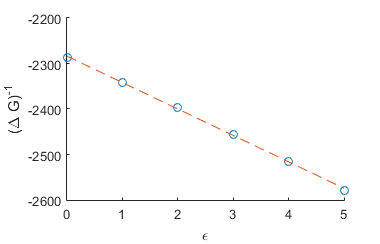
\includegraphics[width=0.5\textwidth]{fig_res/res_DG_tempdep_2}\label{fig:DG_tempdep}
	}
	\caption{(a) Plot of $J_{ss}$ for data sets $\epsilon=0$ to $\epsilon=5$ (blue circles), along with quadratic fit in semi-log space (red dashed line) showcasing faster than exponential decrease. Error bars are not visible at this scale. (b) Plot of $(\Delta G)^{-1}$ as a function of temperature $\Delta B$, over the range of temperatures for the data sets $\epsilon=0$ to $\epsilon=5$. Blue circles are calculated values, red dashed line is a linear fit.}
\end{figure}

Figures \ref{fig:res_Jss} plots $J_{ss}$ for the data sets, on a semi-log plot. Also shown is a quadratic fit in semi-log space to demonstrate faster than exponential decrease of $J_{ss}$ as effective temperature $\Delta B$ increases. To compare this change in rate to equation \ref{eq:nuc_Jss_scaling}, we only consider the effect of the exponential terms in that equation. As discussed in section \ref{sec:nuc_cnt_pfc}, we take $k_B T$ in the exponents to be constant as it depends on $N_a$, and $\Delta G_A$ and $\gamma$ to be positive and decreasing as $\Delta B$ increases. We must then turn to $\Delta G$ to explain the observed change in $J_{ss}$. Figure \ref{fig:DG_tempdep} plots $(\Delta G)^{-1}$ over the range of $\Delta B$ corresponding to the data sets, by estimating $\Delta G = F_s - F_l$ with the liquid and solid bulk energy densities obtained from section \ref{sec:pfc_phasediag}. We observe that this plot varies approximately linearly with $\Delta B$, meaning $\Delta G$ can only account for at most exponential decrease, not faster than exponential. This suggests either that the CNT definitions of $\Delta G$ and $\gamma$ are inadequate for the PFC model, as mentioned in section \ref{sec:nuc_cnt_pfc}, or that the linear fit in the geometric construction used to obtain $J_{ss}$ was not at the true asymptote, which might have resulted in a lower bound for $J_{ss}$ that is less accurate for the data sets of lower $\epsilon$.

We note that experimental predictions and results for physical materials do not disagree with the form of the $J_{ss}$ plot we obtained. Figure \ref{fig:res_Jss_examples} shows steady state homogeneous nucleation rates for water and a CuCo alloy, reproduced from experimental papers. We observe a faster than exponential decrease as temperature increases on the right parts of these plots. We are unable to access the equivalent of the left parts of these plots using the PFC model described in this work, as the decrease in nucleation rate as temperature decreases in these parts of the plots requires a model with a temperature-dependent solute mobility parameter.

\begin{figure}[!h]
	\centering
	\subfloat[]
	{
		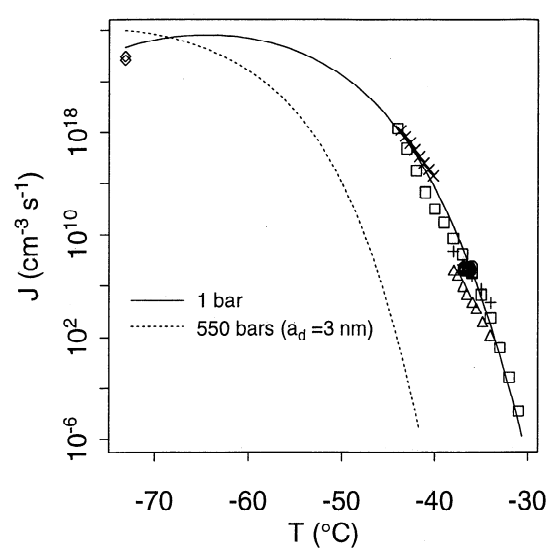
\includegraphics[width=0.5\textwidth]{fig_res/res_Jss_ex_water}
	}
	\subfloat[]
	{
		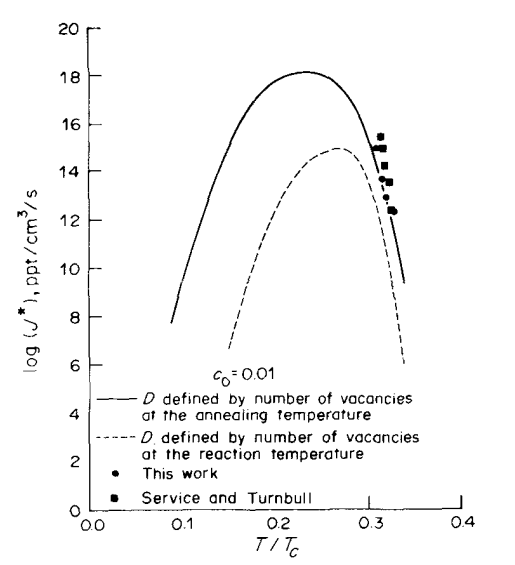
\includegraphics[width=0.5\textwidth]{fig_res/res_Jss_ex_cuco}
	}
	\caption{(a) Predicted steady state homogeneous nucleation rate for supercooled water, with some experimental results shown as symbols along the plot. Reproduced from \cite{jeffery97}. (b) Predicted steady state homogeneous nucleation rate for a CuCo alloy, with some experimental results shown as symbols along the plot. Reproduced from \cite{legoues84}.}\label{fig:res_Jss_examples}
\end{figure}

Figures \ref{fig:res_tinc} plots $t^*$ for the data sets. We observe that $t^*$ increases with temperature $\Delta B$. Comparing to equation \ref{eq:nuc_tinc_scaling}, the exponential term in that equation can not be the source of that increase under the assumptions that $k_B T$ depends on $N_a$ and $\Delta G_A$ decreases with one or both of the temperature parameters of the PFC model. As figures \ref{fig:res_I_datasets} and \ref{fig:res_I_datasets_examples} demonstrate that, for our datasets, the incubation time is larger than the time taken for $J^*(t)$ to increase from zero to $J_{ss}$, we can safely assume that $K>0$ in equation \ref{eq:nuc_tinc_scaling}. Recall that $\gamma$ in the PFC model decreases slowly with $\Delta B$. We take that $\gamma$ decreases much more slowly than $\Delta G$ increases, a fact that can be seen to hold due to the faster than exponential decrease of our calculated $J_{ss}$ despite a factor of $-\gamma^2/\Delta G$ in an exponential term in equation \ref{eq:nuc_Jss_scaling}. We can then conclude that the pre-exponential terms in equation \ref{eq:nuc_tinc_scaling} agree with an increase of $t^*$ with $\Delta B$ as observed, though no exact fit is attempted. This increase also agrees with the predictions for physical materials (for example, see the so-called TTT curves in \cite{legoues84}), again for temperatures where temperature-dependence of solute mobility is negligible.

\begin{figure}[h]
\centering
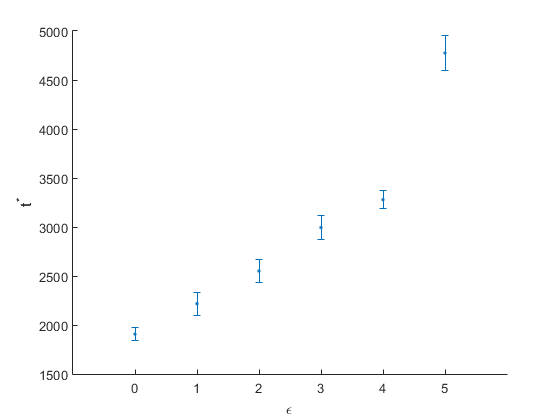
\includegraphics[width=0.8\textwidth]{fig_res/res_tinc}
\caption{Plot of $t^*$ for data sets $\epsilon=0$ to $\epsilon=5$.}\label{fig:res_tinc}
\end{figure}

%%%%%%%%%%%%%%%%%%%%%%%%%%%%%%%%%%%%%%%%%%%%%%%%%%%%%%%%%%%%%%%%%%%%%%%%%%%%%%%%%%%%
\section{Behavior of wave modes during nucleation}\label{sec:res_wavemodes}

In CNT, the stochastically appearing grains are assumed to form with the same lattice structure as the final solid phase. However, as the PFC model is based on a continuous density field, it is feasible that free-standing planar density waves or other non-lattice structures might temporarily appear in simulated PFC systems, especially during the early formation stages of solid grains. To assess whether such occurrences were prevalent in the simulation runs used to obtain the data sets of section \ref{sec:res_longtime}, we use the field filtering method developed in section \ref{sec:num_wave} to examine the growth of separate wave modes during the early formation of a few grains.

To obtain the relative amplitude growth of wave modes at points where nucleation events occur, the filtering process is applied every few time steps of a nucleation-rate simulation, for a range of rotation angles. The value of the filtered field at positions where nucleation occurs is then stored. Figure \ref{fig:res_wavelet_fieldvalues} plots the value of the filtered field at a specific point where nucleation was seen to occur, for a range of times and wavelet rotation angles, in a PFC system with model parameters corresponding to data set $\epsilon=4$. We see three peaks emerge, corresponding to the three wave modes expected in the final solid bulk. At the final time shown ($t=9000$), the post-critical nucleus is known to have grown to a size much larger than the critical size, indicating that the values of the field at that time is that of the final solid. We note that the height of the three peaks in the final solid are not equal as would be expected from the one-mode expansion of section \ref{sec:pfc_1mode}. This is assumed to be due to numerical error, as the square numerical grid has 4-fold symmetry while the final lattice structure has 6-fold symmetry, leading to slight numerical anisotropy in the application of the convolution filter.

 \begin{figure}[h]
	\centering
	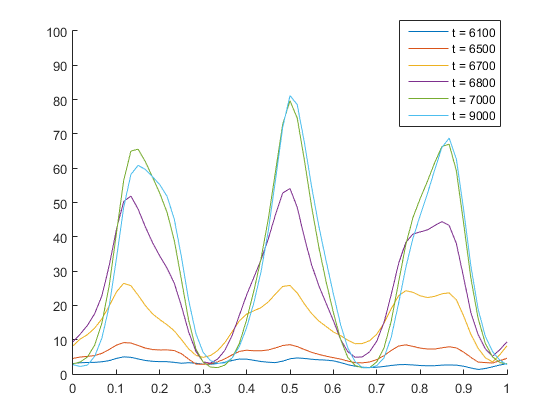
\includegraphics[width=0.7\textwidth]{fig_res/convField_byAngle}
	\caption{Value of the filtered field (y-axis) as a function of wavelet rotation angle (x-axis), for a range of times beginning before nucleation occurs and ending after the post-critical nucleus has grown to a size much larger than the critical size. The x-axis is in fractions of $\pi$.}\label{fig:res_wavelet_fieldvalues}
\end{figure}

Once the angles for the peaks of the filtered field are known at late times, we can plot the growth with time of the field for only these three angles starting from early times. Figure \ref{fig:res_convfield_nuc} plots the growth of these peaks for two nucleation events, with parameters corresponding to data set $\epsilon=0$. The values are normalized with respect to the maximum value attained by each peak, to account for the mentioned inequality of the peaks at late time due to numerical anisotropy. We also examined other nucleation events and obtained similar plots.


\begin{figure}[!h]
	\centering
	\subfloat[]
	{
		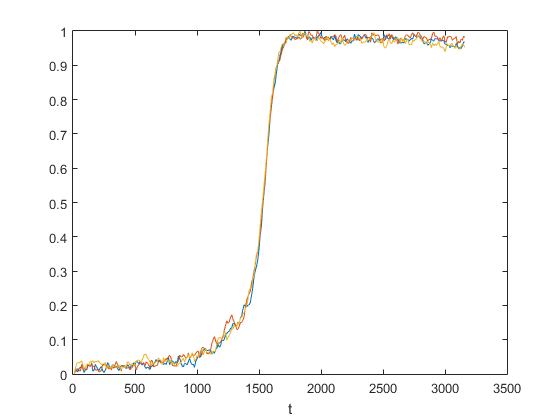
\includegraphics[width=0.47\textwidth]{fig_res/res_convfield_nuc_set20_event1}
	}\label{fig:res_convfield_nuc_a}
	\subfloat[]
	{
		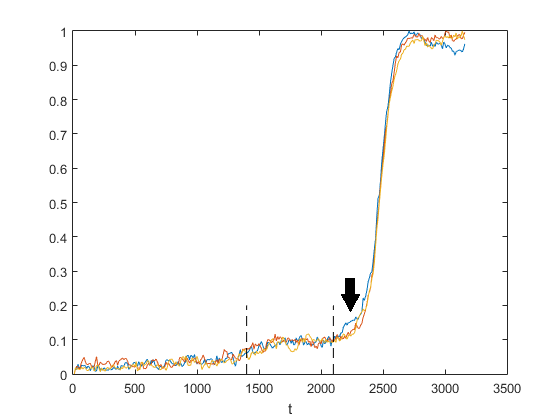
\includegraphics[width=0.47\textwidth]{fig_res/res_convfield_nuc_set20_event30_mod}\label{fig:res_convfield_nuc_b}
	}
	\caption{Normalized values of the filtered field at the angles where the three late time peaks are found (corresponding to the three shown colors), as a function of time, for two separate nucleation events in the same simulated system.}\label{fig:res_convfield_nuc}
\end{figure}

\begin{figure}[!h]
	\centering
	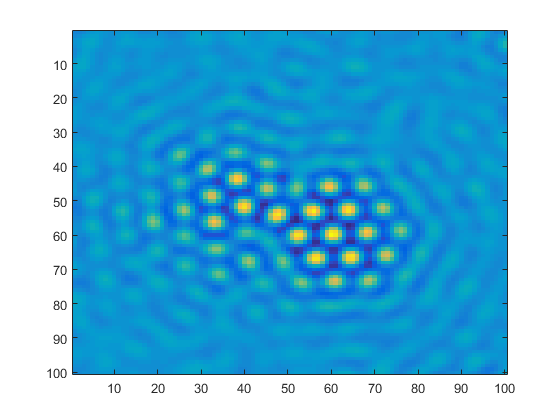
\includegraphics[width=0.6\textwidth]{fig_res/res_convfield_examplegrain}
	\caption{Density field of the grain from which peak filtered field values shown in figure \ref{fig:res_convfield_nuc_b} where obtained, at time $t=2550$. Axes indicate grid points.}\label{fig:res_convfield_examplegrain}
\end{figure}

The filtered field values at the three peak positions appear to vary in tandem during the majority of the process (up to the order of thermal fluctuations). This leads us to conclude that, at least for the parameter ranges of the data sets of section \ref{sec:res_longtime}, nucleation in the PFC model exhibits atomic lattice structure even during the relatively early parts of grain formation. However, a minority of examined grains display unexpected behavior of the field values at the three peaks, such as the grain corresponding to figure \ref{fig:res_convfield_nuc_b}. In that figure, the black arrow points to a relatively large fluctuation of only one mode that appears to precede the rapid growth of all three modes. The dashed lines denote a range of time where the three modes' growth seems to be delayed at a value higher than the background value, yet lower than the final solid value. We believe these behaviors are due to a few grains forming with more complex forms, unaccounted for in our assumptions. Figure \ref{fig:res_convfield_examplegrain} shows the grain corresponding to figure \ref{fig:res_convfield_nuc_b}. We observe that this grain appears to exhibit two separate lattice orientations. This is possibly due to it being formed from two grains that merged into one at an earlier time. Another possible explanation is the existence of a precursor non-crystalline phase or preferred structure that precedes criticality. The competition between these separate lattice orientations might explain the delay observed in \ref{fig:res_convfield_nuc_b}, as well as the single mode fluctuation before the final rapid growth.

These results indicate that the developed wave mode analysis method requires further refinement to be able to distinguish such edge cases. They also offer more insight into the difficulties involved in applying CNT to nucleation in the PFC model, as these complex-structured grains violate CNT's no-interaction or crystalline-structure assumptions, likely extending the required time for these grains to achieve criticality as their lattice structures stabilizes.






%%%%%%%%%%%%%%%%%%%%%%%%%%%%%%%%%%%%%%%%%%%%%%%%%%%%%%%%%%%%%%%%%%%%%%%%%%%%%%%%%%%%
\section{Critical nucleus curves for chosen parameters}\label{sec:res_testnuc}

We numerically calculate the `critical nucleus curves' for the parameters of data sets $\epsilon=0$ to $\epsilon=5$, using the method described in section \ref{sec:num_testnuc}. Figure \ref{fig:res_criticality} shows these curves. We observe that, as $\epsilon$ (equivalently, the effective temperature $\Delta B$) increases, the curves shift along both the relative order axis (y-axis) and size axis (x-axis). The shift along the size axis agrees with the basic prediction of CNT that critical radius must increase with temperature. However, CNT does not account for the shift along the order axis, as it assumes the lattice structure in the interior of the grain is always the same as that of the final solid. Further, the precise path that a forming grain would take through the $(r_1,r_2)$ parameter space before becoming a post-critical nucleus can not be predicted by CNT, instead requiring at least a 2 parameter theory similar to that developed in \cite{lutsko15} for the case of nucleation in globular protein systems. We expect that the most likely path to criticality will depend on a balance between statistically probable fluctuation amplitude and diminishing correlation at range: A critical nucleus of too small radius is unlikely to form due to the exponentially decreasing odds of obtaining a sufficiently large fluctuation as required field amplitude increases, while a critical nucleus of too large radius is unlikely to form before smaller grains because the spatially conserved density fluctuations in the system limit the rate at which mass and information of the forming lattice structure can propagate at large distances.

\begin{figure}[h]
	\centering
	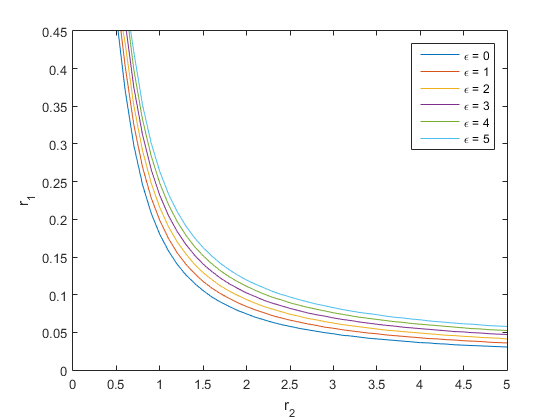
\includegraphics[width=0.8\textwidth]{fig_res/res_criticality}
	\caption{Critical nucleus curves for data sets $\epsilon=0$ to $\epsilon=5$. Recall that $r_1$ is a ratio that scales the amplitude of the density field of the grain, while $r_2$ scales the radius of the Gaussian-shaped grain.}\label{fig:res_criticality}
\end{figure}


%%%%%%%%%%%%%%%%%%%%%%%%%%%%%%%%%%%%%%%%%%%%%%%%%%%%%%%%%%%%%%%%%%%%%%%%%%%%%%%%%%%%
\section{Nucleation at different noise amplitudes}\label{sec:res_diffnoise}

The data sets of section \ref{sec:res_longtime} allowed the comparison of nucleation in the PFC model to CNT as the effective temperature $\Delta B$ varied. However, the chosen range of $\Delta B$ was too small to warrant a non-negligible change of $N_a$. It is of interest to examine the behavior of nucleation as a function of noise amplitude alone, to see whether our assumptions about the temperature dependence of the various values in equations \ref{eq:nuc_Jss_scaling} and \ref{eq:nuc_tinc_scaling} were warranted. In this section, we relax the requirement found by the authors of \cite{kocher16} on the noise amplitude parameter $N_a$, allowing it to be varied independently of $\Delta B$ over multiple new data sets. We stress that the new data sets' $J_{ss}$ and $t^*$ curves are not expected to vary as would be predicted for a physical system, as decoupling the choice of $N_a$ from $\Delta B$ effectively leads to the thermal fluctuations being unphysical.

We generate six new data sets with fixed model parameters $n_o=0.207$, $B^x=0.4$, and $\Delta B=0.1650$, and with increasing noise amplitude $N_a=0.030+0.002\kappa$ for $\kappa$ an integer from 0 to 5 corresponding to the six sets in order from first to last. Note that all these data sets would have the same critical nucleus curve as found for data set $\epsilon=0$ in section \ref{sec:res_testnuc}, since the critical nucleus curves depend on parameters $n_o$, $B^x$, and $\Delta B$, but not on $N_a$.

We repeat the procedure of section \ref{sec:res_longtime} for the new data sets. Figure \ref{fig:res_I_datasets_newnoise} plots their post-critical nuclei densities $I^*(t)$. Figure \ref{fig:res_I_datasets_examples_newnoise} demonstrates the geometric constructions for two of the data sets. Figures \ref{fig:res_Jss_newnoise} and \ref{fig:res_tinc_newnoise} plot $J_{ss}$ and $t^*$ for these data sets respectively. Note that the x-axes for these two plots are in terms of $T_r=N_a^2/2$, the fluctuation temperature obtained from the fluctuation-dissipation theorem as mentioned in section \ref{sec:pfc_dynamics}.


\begin{figure}[!h]
		\centering
	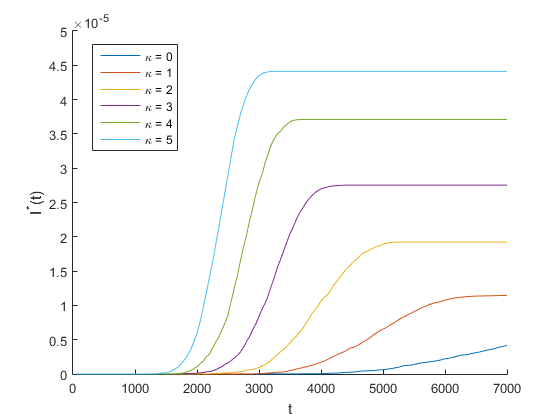
\includegraphics[width=0.7\textwidth]{fig_res/res_I_datasets_newnoise}
	\caption{The post-critical nuclei densities for data sets $\kappa=0$ to $\kappa=5$.}\label{fig:res_I_datasets_newnoise}
	\centering
	\subfloat[]
	{
		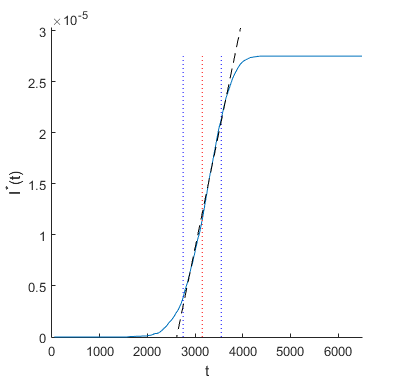
\includegraphics[width=0.5\textwidth]{fig_res/res_Ik2}
	}
	\subfloat[]
	{
		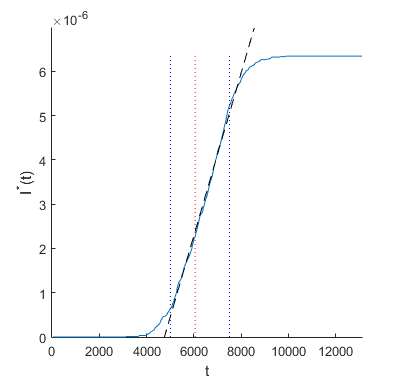
\includegraphics[width=0.5\textwidth]{fig_res/res_Ik5}
	}
	\caption{The geometric construction used to obtain $J_{ss}$ and $t^*$. The vertical blue dotted lines indicate the range of time taken to correspond to the asymptote. The dashed black line is the linear fit over that time range. Also shown as a vertical red dotted line is the time at which 10\% of the initial liquid volume has solidified. (a) Data set $\kappa=2$, giving $J_{ss}=(2.26\pm 0.09)\times10^{-8}$ and $t^*=2600\pm 200$. (b) Data set $\kappa=5$, giving $J_{ss}=1.84\pm 0.04)\times10^{-9}$ and $t^*=4800\pm 200$. The errors on these values are from the uncertainty on the linear fit.}\label{fig:res_I_datasets_examples_newnoise}
\end{figure}


Considering only the exponential terms of equation \ref{eq:nuc_Jss_scaling}, and recalling that $\gamma$ and $\Delta G$ only vary with $\Delta B$, the observed variation of $J_{ss}$ is expected to be due to $\Delta G_A$ and $k_B T$. Setting $k_B T = T_r$, we attempt a fit of form $A_1\exp(-A_2/T_r)$ where $A_1$ and $A_2$ are fit parameters to the plot of $J_{ss}$, as shown on figure \ref{fig:res_Jss_newnoise}. The fit suggests agreement between equation \ref{eq:nuc_Jss_scaling} and our results, assuming $\Delta G_A+\pi\gamma^2/(-\Delta G)$ varies slowly over the considered range of $T_r$.

As for incubation time, again due to $\gamma$ and $\Delta G$ not varying for these data sets, equation \ref{eq:nuc_tinc_scaling} indicates that $t^*$ would scale as $\exp(+\Delta G_A/k_B T)$ with $\Delta G_A$ decreasing with temperature and setting $k_B T = T_r$. Figure \ref{fig:res_tinc_newnoise} suggests agreement with equation \ref{eq:nuc_tinc_scaling}, though a specific fit was not attempted as the error bars allow both exponential as well as linear fits to be plausible.

\begin{figure}[h]
	\centering
	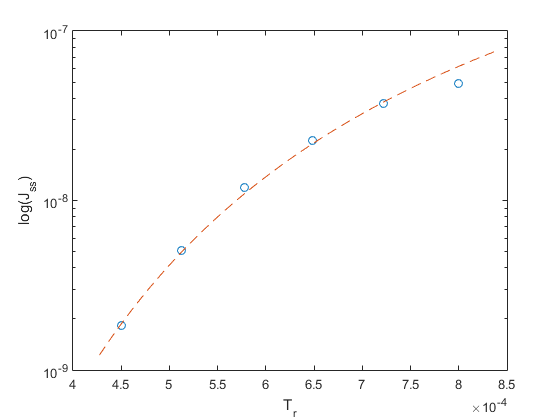
\includegraphics[width=0.8\textwidth]{fig_res/res_Jss_newnoise_Trfit}
	\caption{Plot of $J_{ss}$ for data sets $\kappa=0$ to $\kappa=5$ (blue circles), along with a fit of form $A_1\exp(-A_2/T_r)$ for fit parameters $A_1=5.57\times 10^{-6}$ and $A_2=0.0036$ (red dashed line). Error bars are not visible at this scale. }\label{fig:res_Jss_newnoise}
\end{figure}

\begin{figure}[h]
	\centering
	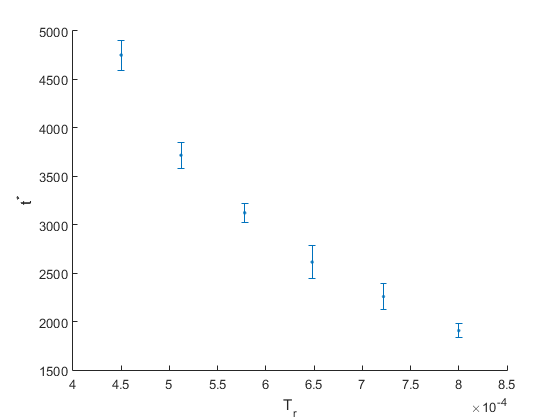
\includegraphics[width=0.8\textwidth]{fig_res/res_tinc_newnoise}
	\caption{Plot of $t^*$ for data sets $\kappa=0$ to $\kappa=5$.}\label{fig:res_tinc_newnoise}
\end{figure}



%%%%%%%%%%%%%%%%%%%%%%%%%%%%%%%%%%%%%%%%%%%%%%%%%%%%%%%%%%%%%%%%%%%%%%%%%%%%%%%%%%%%










